\documentclass[a4paper]{article}
\usepackage[utf8]{inputenc}
\usepackage{a4wide}
\usepackage{appendix}
\usepackage[T1]{fontenc}
\usepackage[pdftex]{graphicx}

\title{\Huge A* Pathfinding Acceleration with use of Auto-Generated Waypoints for Grid Traversal in a Static Environment}
\author{Fredrik Olsson, Magnus Nyqvst}
\date{\today} 

\begin{document}
\pagenumbering{gobble}
\maketitle
\newpage
\thispagestyle{empty}
\paragraph{Abstract--}
Sammanfattar rapporten
Varför är vår rapport värd att läsa?
Syfte, metod
Viktiga resultat och slutsatser Nyckelord
“Tänk på att detta skall kunna läsas fristående”

\tableofcontents
\listoffigures
\newpage
\pagenumbering{arabic}
\twocolumn
\section{Introduction}
Pathfinding is a fundamental part of games \cite{dynaPF15}\cite{roboGame15} and it is often supplemented by a waypoint graph to make traversal of a given region easier \cite{dynaPF15}. Every node in a waypoint graph is called a waypoint and they represent key locations in the region \cite{dynaPF15}. Each waypoint has edges towards other waypoints to where an object can travel through without risk of colliding with the surroundings \cite{dynaPF15}.
	
In this paper, we propose a method to reduce execution time of the A* pathfinding algorithm. We improve our previously implemented A* algorithm with automatically generated and connected waypoints in a two-dimensional grid coordinate system. The waypoint generation is done in two steps. First, we generate a waypoint for each corner of an obstacle. Second, we check connections for every waypoint by sending a ray towards all other waypoints in the region. The waypoints are connected if the rays path is unblocked. Our waypoint generation method is heavily influenced by the one suggested in the work of Weiping et al. \cite{dynaPF15}.
	
Executing pathfinding in dynamic environments is more challenging than in static environments \cite{dynaPF15}, and this study is therefore limited to completely static environments. The difference between the two terms path and shortest path is significant \cite{heuristicGame15}. We conducted studies of several pathfinding combinations, with and without waypoints, but we decided not to measure the time consumption of the shortest path with only A* pathfinding.
	
A heurstic is a method/algorithm to choice next edge during the traversal of the grid.

This is introduction lol \newline
Syfte \newline
Frågeställning \newline
Hypoteser \newline
Avgränsningar

\section{Related work}
This work is based on Weiping et al. \cite{dynaPF15} work but we've done it in a static environment instead and mixed it with grid based traversal with A*.

\section{Method}
The autogeneration of waypoints are very much inspired by the work done in \cite{dynaPF15}. Becouse our environment is 2D and all geometry are boxes, we place all boxes inside large boxes to devide the blocked parts of the maps into regions. Every corner of every region gets a waypoint, offseted with .5 of a tile size. If a waypoint shares a tile with another waypoint
the second waypoint will not be added.
	
To connect the waypoint to eachother, we shoot a ray from every waypoint to every waypoint (sqr(n)) and traverse a qaudtree to find an intersection with geometry. If an intersection is found, no connection will be added. [EDGE REFERSEN FREDRIK PLES FIX]. Each edge gets assigned a cost that is equal to the distance between the waypoints squared.

Now all unblocked tiles gets divided into subregions. Each subregion belongs to a waypoint and each tile gets assigned to the region with the closest visible waypoint. This is to know which waypoint to start the path from during the waypoint traversal thinghy.

When a path is requested, the start and end poisiton gets translated into tiles. From these tiles, the stat region- and end region waypoint gets extracted and the waypoint traversal algorthim starts. To travese the waypoints we use an A* algortihm with a closed list and open list to create a thing we call tileChain. this tilechains represents the tiles the waypoints stand on.
When we have the tilechain we send theses "sub-paths" into the classic A* algorithm (closed list, early exploration list and open list). Each of these paths are so short so the Tile A* traversal is very short.

To sample our data we have done 27 different test on three different maps. These maps vary in size and structure. Edgy is a the smallest map with 9085 tiles and a blockrate of 46.5 \%, 214 waypoints with 2228 connections. Edgy2 is constructed the same as Edgy, but greater in size, 26550 tiles with a blockrate of 48.4 \%, 658 waypoints with 6458 connections, its basicaly Edgy but repeated. The biggest map is UMAP2, it is constructed as two "U"s faced away from eachother. This map has 335748 tiles with a blockrate of 8 \%, 179 waypoints with 2038 connections.

On each map, we have selected nine different paths and done three test per path with different heuristics, Pure Distance, Manhattan Distnace (REFTO MH) and Stanford Distance (REF TO SD).
Each setting on each path were tested 100 times each. To get the delta time changes between waypoint traversal and A* tile traversal we took the avarage total time of each test.
The Pure Distance heuristic simply checks the pure distance to the goal to choose the next edge to traverse. The paths of choice is not biast, they are chosen to favor all pathfinding methods.

We have discovered that our solution to waypoint generation gives a huge advantage on bigger maps. The waypoint traversal scales much better then raw A*. Also, waypoint traversal works excelent in edge cases, where A* compleatly fails.
When traversing on a small map, the edge cases are not enoght motivation to implement automatilcly gnererated waypoints due to the overhead the waypoints adds to the algorithms.

We have limited ourselves to only compare traversal time and we have not taken into account loading time for the map, memmory usage nor dynamic enviroments.
	
We decided to remove the best waypoint path because we have nothing to compare them with. We could not do the tests with the best tile path due to it took hours to compleate the traversal.
	
We hav not taken into account that the paths may be "un natrual" for the viewer during this work. The goal was to find a way to find paths in a static enviroment in real time.

\section{Result}

The results show that traversing the grid with our automaticaly generated waypoint apporach is much more scalable than using the A* algorithm raw. This also holds true when changing the heuristics for the traversing algorithms.
	
In the smallest map, Appendix~\ref{ap.edgy}, it is cheaper to simply use A* to generate the path due to the added overhead using waypoints. Waypoint traversal is superior to A* pathfinding when the maps increase in size and complexity.
	
On the maps Edgy2, Appendix~\ref{ap.edgy2}, and UMAP2, Appendix~\ref{ap.umap2}, which are much greater in size compared to Edgy we see from the results that in almost all the paths traversing the waypoints first to direct the A* takes much less time on almost every path. In the charts we can see that in some of the paths
A* is faster by itself than with use of waypoints. This is because these paths are short or straight, with no or few blocked tiles in the way of the pathing.
		
In the comparison diagrams the color green , purple and red boxes represents traversal with waypoints with the Pure Distance- , Manhattan Distance- and Standford distance heuristic.
The color blue, cyan and brown colors represent traversal with pure A* tile traversal with the Pure Distance- , Manhattan Distance- and Standford distance heuristic.
The  X-axis is the nine different paths and the Y-axis is time in milliseconds.

\begin{figure}[h!]
\centering
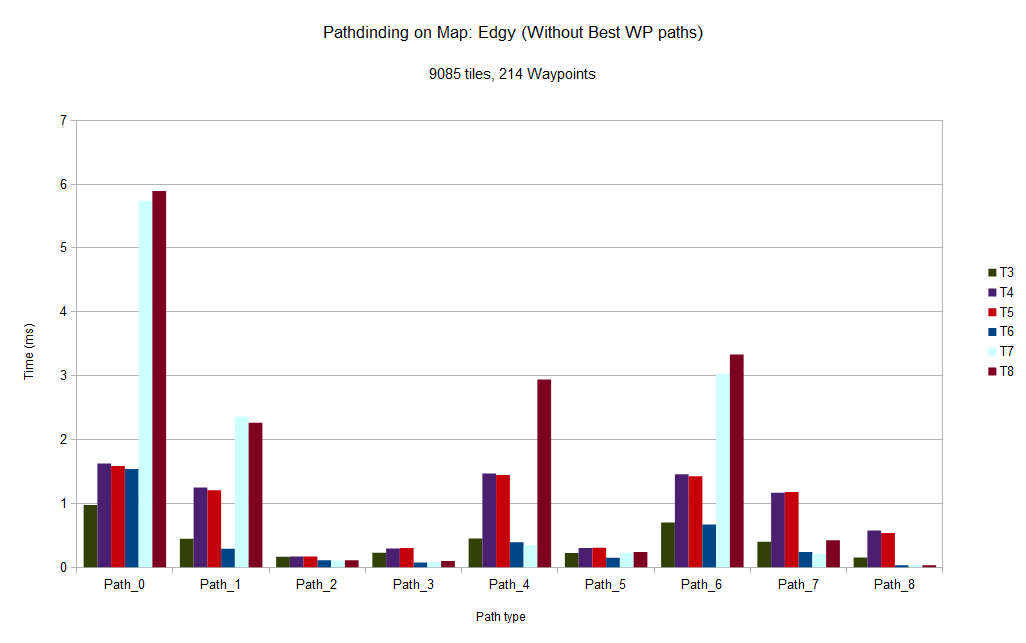
\includegraphics[width=0.5\textwidth,height=\textheight,keepaspectratio]{ChartsAndFigures/Edgy_d2.png}
\caption{Edgy Compare Diagram}
\label{fig:Edgy_d2}
\end{figure}
\begin{figure}[h!]
\centering
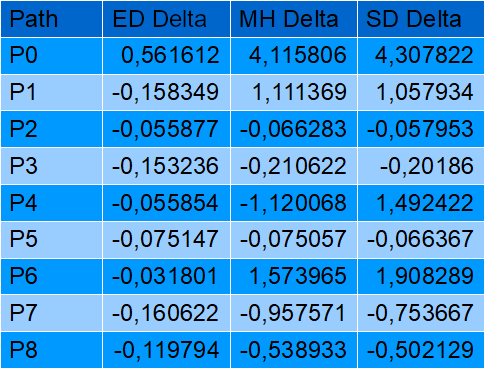
\includegraphics[width=0.5\textwidth,height=\textheight,keepaspectratio]{ChartsAndFigures/Edgy_timeTable.png}
\caption{Edgy Time Table}
Delta time gain using waypoints in milliseconds.
\label{fig:Edgy_cd}
\end{figure}


On the Edgy map, in Figure \ref{fig:Edgy_d2}, we see all tests compared with eachother. Its easy to see that in most cases, using only tile traversal is better than using waypoint traversal.
The average gain time can be seen in Figure \ref{fig:Edgy_cd} and in almost all cases we loose time when traversing with waypoints.
	
\begin{figure}[h!]
\centering
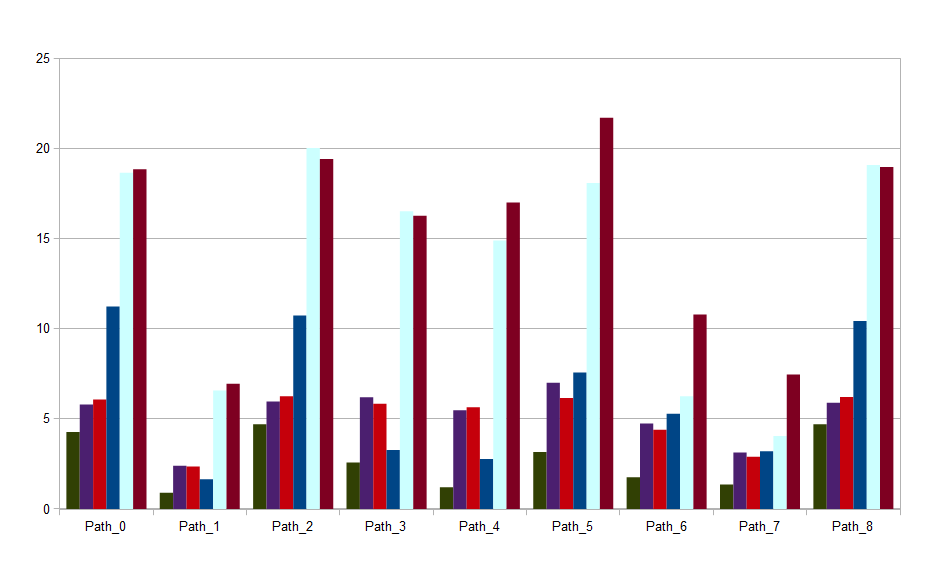
\includegraphics[width=0.5\textwidth,height=\textheight,keepaspectratio]{ChartsAndFigures/Edgy2_d2.png}
\caption{Edgy2 Compare Diagram}
\label{fig:Edgy2_d2}
\end{figure}

\begin{figure}[h!]
\centering
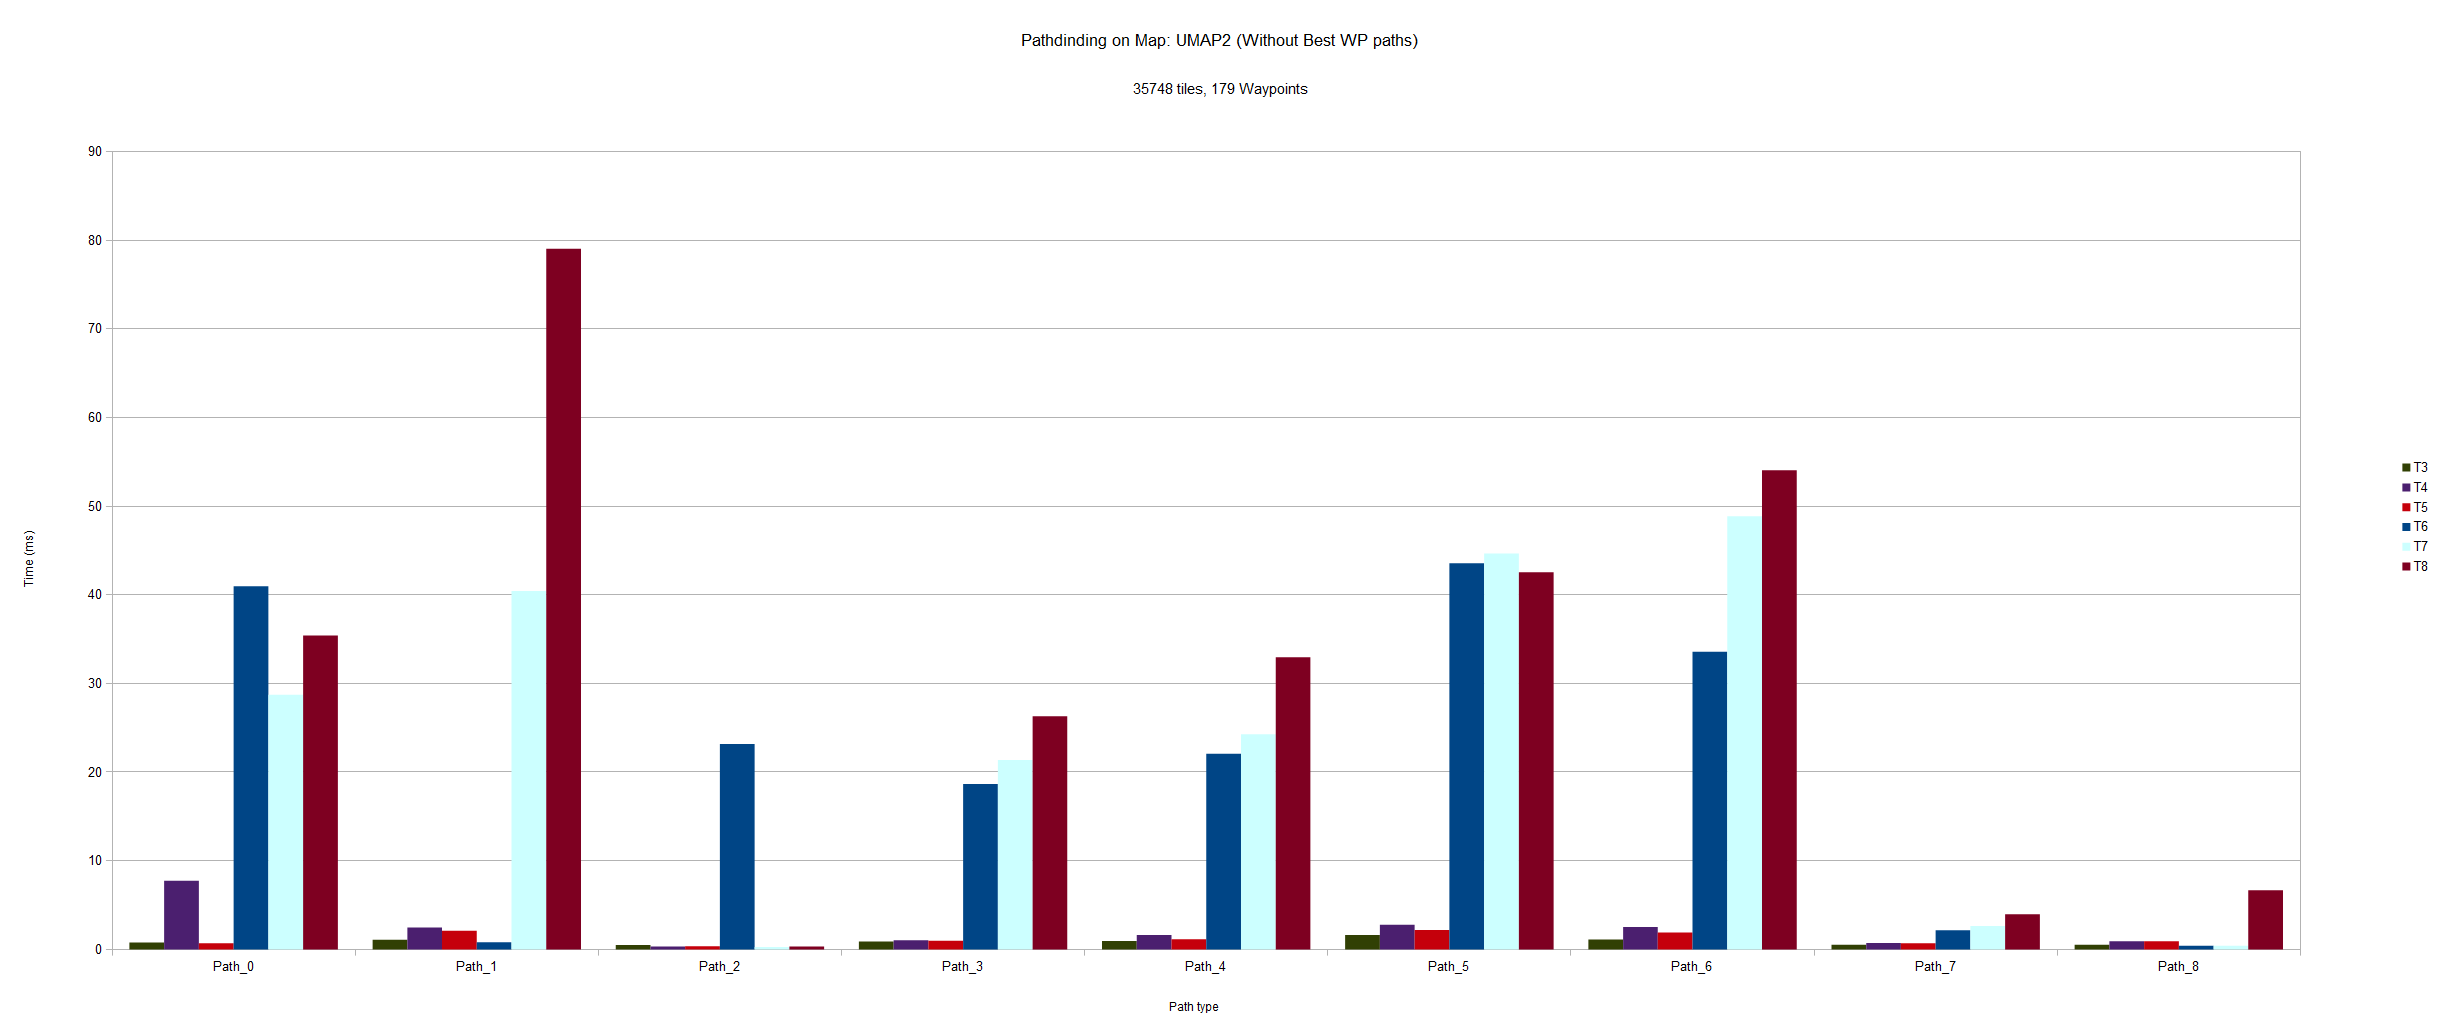
\includegraphics[width=0.5\textwidth,height=\textheight,keepaspectratio]{ChartsAndFigures/UMAP2_d2.png}
\caption{UMAP2 Compare Diagram}
\label{fig:UMAP2_d2}
\end{figure}

However it is clearly displayed that waypoint traversal is superior to A* pathfinding when the map complexity increases. Both Figure~\ref{fig:Edgy2_d2} and Figure~\ref{fig:UMAP2_d2} prove that the gain increases as the map grows.
Waypoint traversal was up to and above 40 milliseconds faster then A* pathfinding on UMAP2 and this is due to the maps edge case layout. In most cases A* would get stack in one of the U-shapes while searching for the goal, whereas waypoint traversal would quickly exit the rabbit hole and continue in the right direction.

\begin{figure}[h!]
\centering
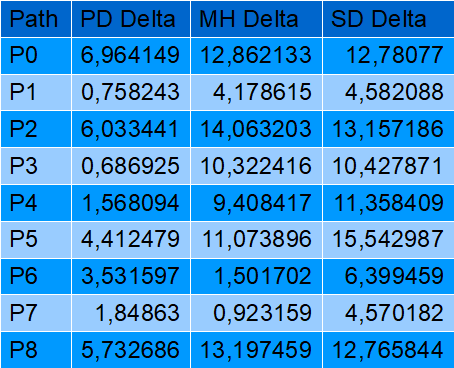
\includegraphics[width=0.5\textwidth,height=\textheight,keepaspectratio]{ChartsAndFigures/Edgy2_timeTable.png}
\caption{Edgy2 Time Table}
Delta time gain using waypoints in milliseconds.
\label{fig:Edgy2_cd}
\end{figure}

\begin{figure}[h!]
\centering
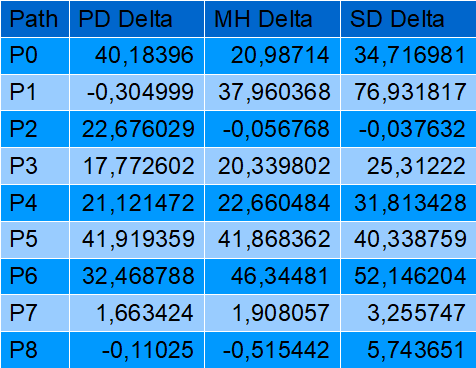
\includegraphics[width=0.5\textwidth,height=\textheight,keepaspectratio]{ChartsAndFigures/UMAP2_timeTable.png}
\caption{UMAP2 Time Table}
Delta time gain using waypoints in milliseconds.
\label{fig:UMAP2_cd}
\end{figure}

The exact avarge gain can be seen in Figure \ref{fig:Edgy2_cd} and Figure \ref{fig:UMAP2_cd}.
	
The validity of the experiemnts have a P value way below 0.05, mosly closely to 0.0.

\section{Discussion}
On smaller maps with a lot of waypoint connections, raw A* is quicker than with our generation of waypoints. But when the map starts to scale, waypoints are significantly better than just A* by itself.
Our results are based on the first path the algorithm finds, not the quickest path. We made some samples when we used the quickest path for waypoint traversal and this were proven to take more time to calculate than using pure A* with the first path found.
It was only on UMAP2 we could get the quickest path for waypoints to get less calcualtion time then just A*, but it is still not real time friendly.

\newpage
\begin{thebibliography}{9}

\bibitem{dynaPF15}
  Weiping Zhu, Daoyuan Jia, Hongyu Wan, Tuo Yang, Cheng Hu, Kechen Qin, Xiaohui Cui,
  \textit{Waypoint Graph Based Fast Pathfinding in Dynamic Environment},
  International Journal of Distributed Sensor Networks, vol. 2015, Article ID 238727, 12 pages,
  August 2015. https://doi.org/10.1155/2015/238727.

\bibitem{roboGame15}
  Zeyad Abd Algfoor, Mohd Shahrizal Sunar, Hoshang Kolivand,
  \textit{A Comprehensive Study on Pathfinding Techniques for Robotics and Video Games},
  International Journal of Computer Games Technology, vol. 2015, Article ID 736138, 11 pages,
  2015. https://doi.org/10.1155/2015/736138.

\bibitem{heuristicGame15}
  Geethu Elizebeth Mathew,
  \textit{Direction Based Heuristic For Pathfinding In Video Games},
  Procedia Computer Science, vol. 47, pp. 262-271,
  2015.

\bibitem{lamport94}
  Leslie Lamport,
  \textit{\LaTeX: a document preparation system},
  Addison Wesley, Massachusetts,
  2nd edition,
  1994.

\end{thebibliography}


\clearpage
\onecolumn
\appendix
\appendixpage
\addappheadtotoc

\section{Map Edgy}\label{ap.edgy}
\centering
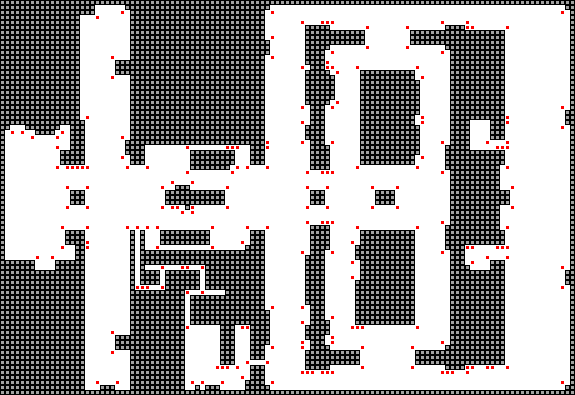
\includegraphics[width=\textwidth,height=\textheight,keepaspectratio]{ChartsAndFigures/Edgy.png}
9085 tiles, 4226 blocked (46.5\%). 214 waypoints with 2228 connections. Gray boxes indicates blocked tiles, Red boxes indicates waypoints and white space are open tiles.

\flushleft
\pagebreak
\section{Map Edgy2}\label{ap.edgy2}
\centering
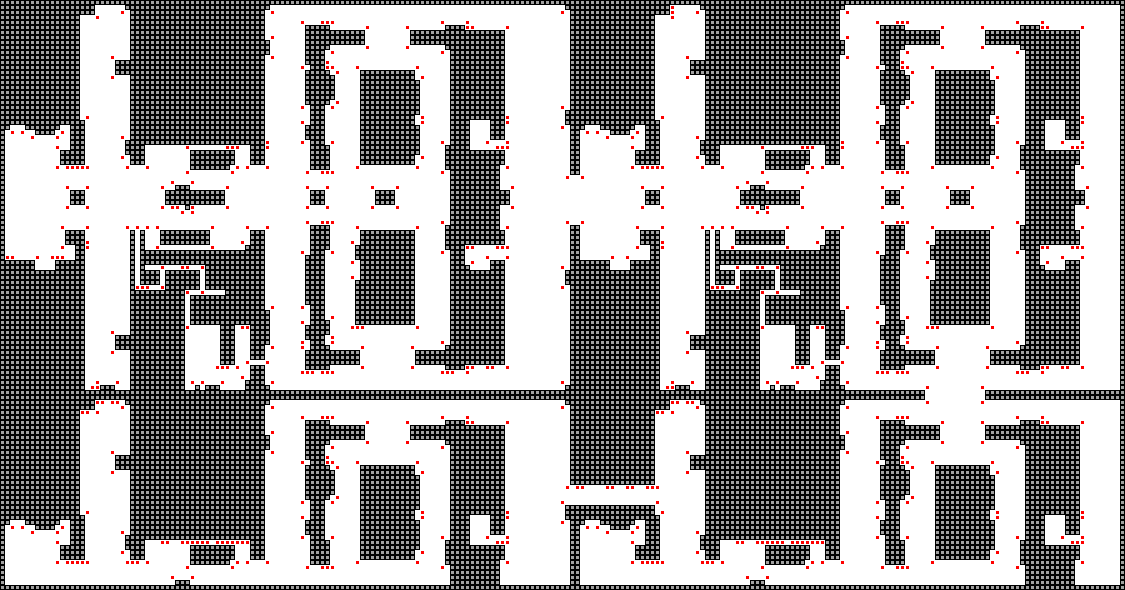
\includegraphics[width=\textwidth,height=\textheight,keepaspectratio]{ChartsAndFigures/Edgy2.png}
26550 tiles, 12854 blocked (48.4\%). 658 waypoints with 6458 connections. Gray boxes indicates blocked tiles, Red boxes indicates waypoints and white space are open tiles.

\flushleft
\section{Map UMAP2}\label{ap.umap2}
\centering
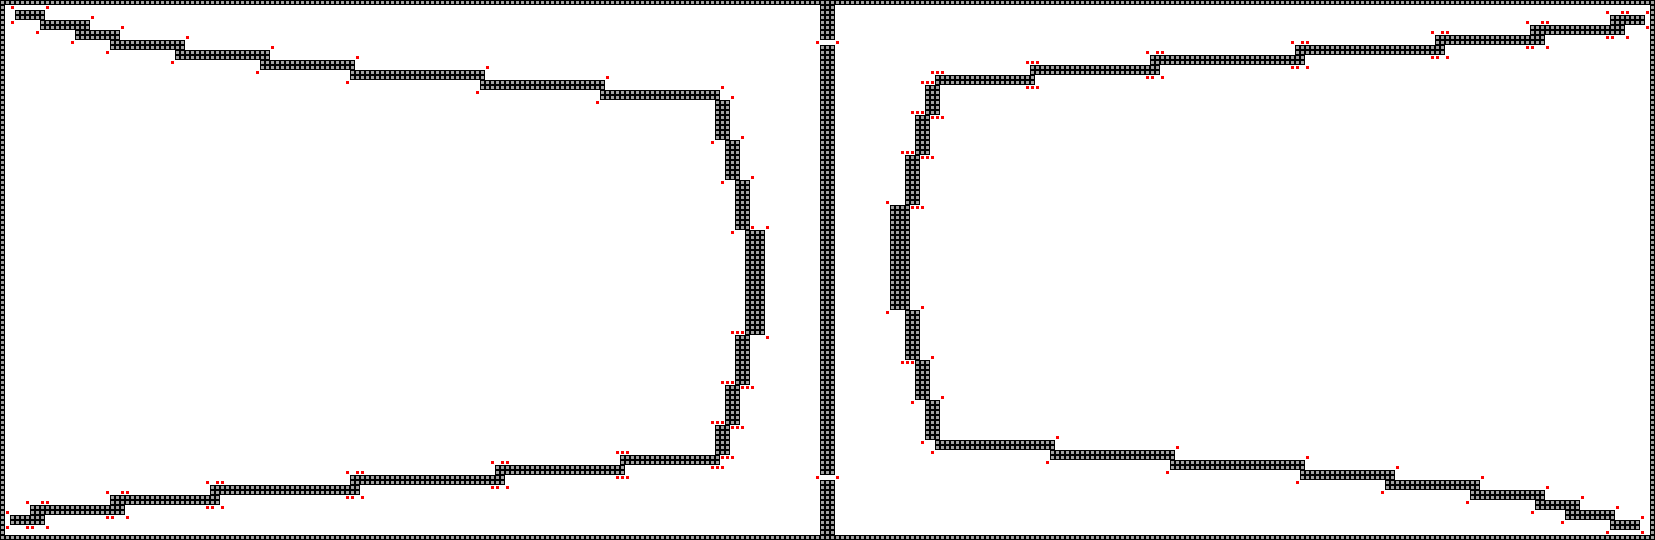
\includegraphics[width=\textwidth,height=\textheight,keepaspectratio]{ChartsAndFigures/UMAP2.png}
35748 tiles, 2890 blocked (8\%). 179 waypoints with 2038 connections. Gray boxes indicates blocked tiles, Red boxes indicates waypoints and white space are open tiles.


\end{document}
